\section{System}
We design the visualization system with modularity and easy of use in mind.
%The initial learning curve and workflow setup cost of the tool are often the most significant barriers for user adaptation.
As a result, we designing the system as a Python library rather than as a monolithic standalone application. 
Just like a plotting library (i.e., matplotlib), the different pieces of the visualization (i.e., matrix based attention encoding) can be accessed individually, which helps ease the initial learning curve. 
The individual components can also be combined in any configuration desired by users via a simple API to better fit into one's workflow.
More importantly, the library-based design allows easy integration with the existing model implemented in Python.
%
To create a visualization, users only need to import the library, create an instance of the visualization object, and specify a set of callback functions, such as generating a prediction, accessing attention, to link the visualization to their NLP models. 

\begin{lstlisting}[language=Python, caption=Code for setting up the visualization system shown in the paper.]
from visPackage import MCModule
from bidaf_src import bidafModelInterface
from NLPutility import translationPerturbation

#initialize machine comprehension model
model = bidafModelInterface(
    wordDict="data/bidaf/squad.word.dict",
    wordVec="data/bidaf/glove.hdf5",
    model="data/bidaf/bidaf.ema")

gen = translationPerturbation()

# visualization components
visLayout = {
  "column":[{"row": ["Paragraph", "AttentionSubMatrix"]},
            {"row": ["AttentionAsymmetric"]}]
  }

#setup interface
modelVis = MCModule(visLayout)

modelVis.setPredictionHook(model.predict)
modelVis.setAttentionHook(model.attention)
modelVis.setReloadModelCallback(model.reloadModel)
modelVis.setSentenceHook(gen.perturbSentence)

#open browser for visualization
modelVis.startServer()
\end{lstlisting}

\begin{figure*}[t]
\centering
\vspace{-2mm}
 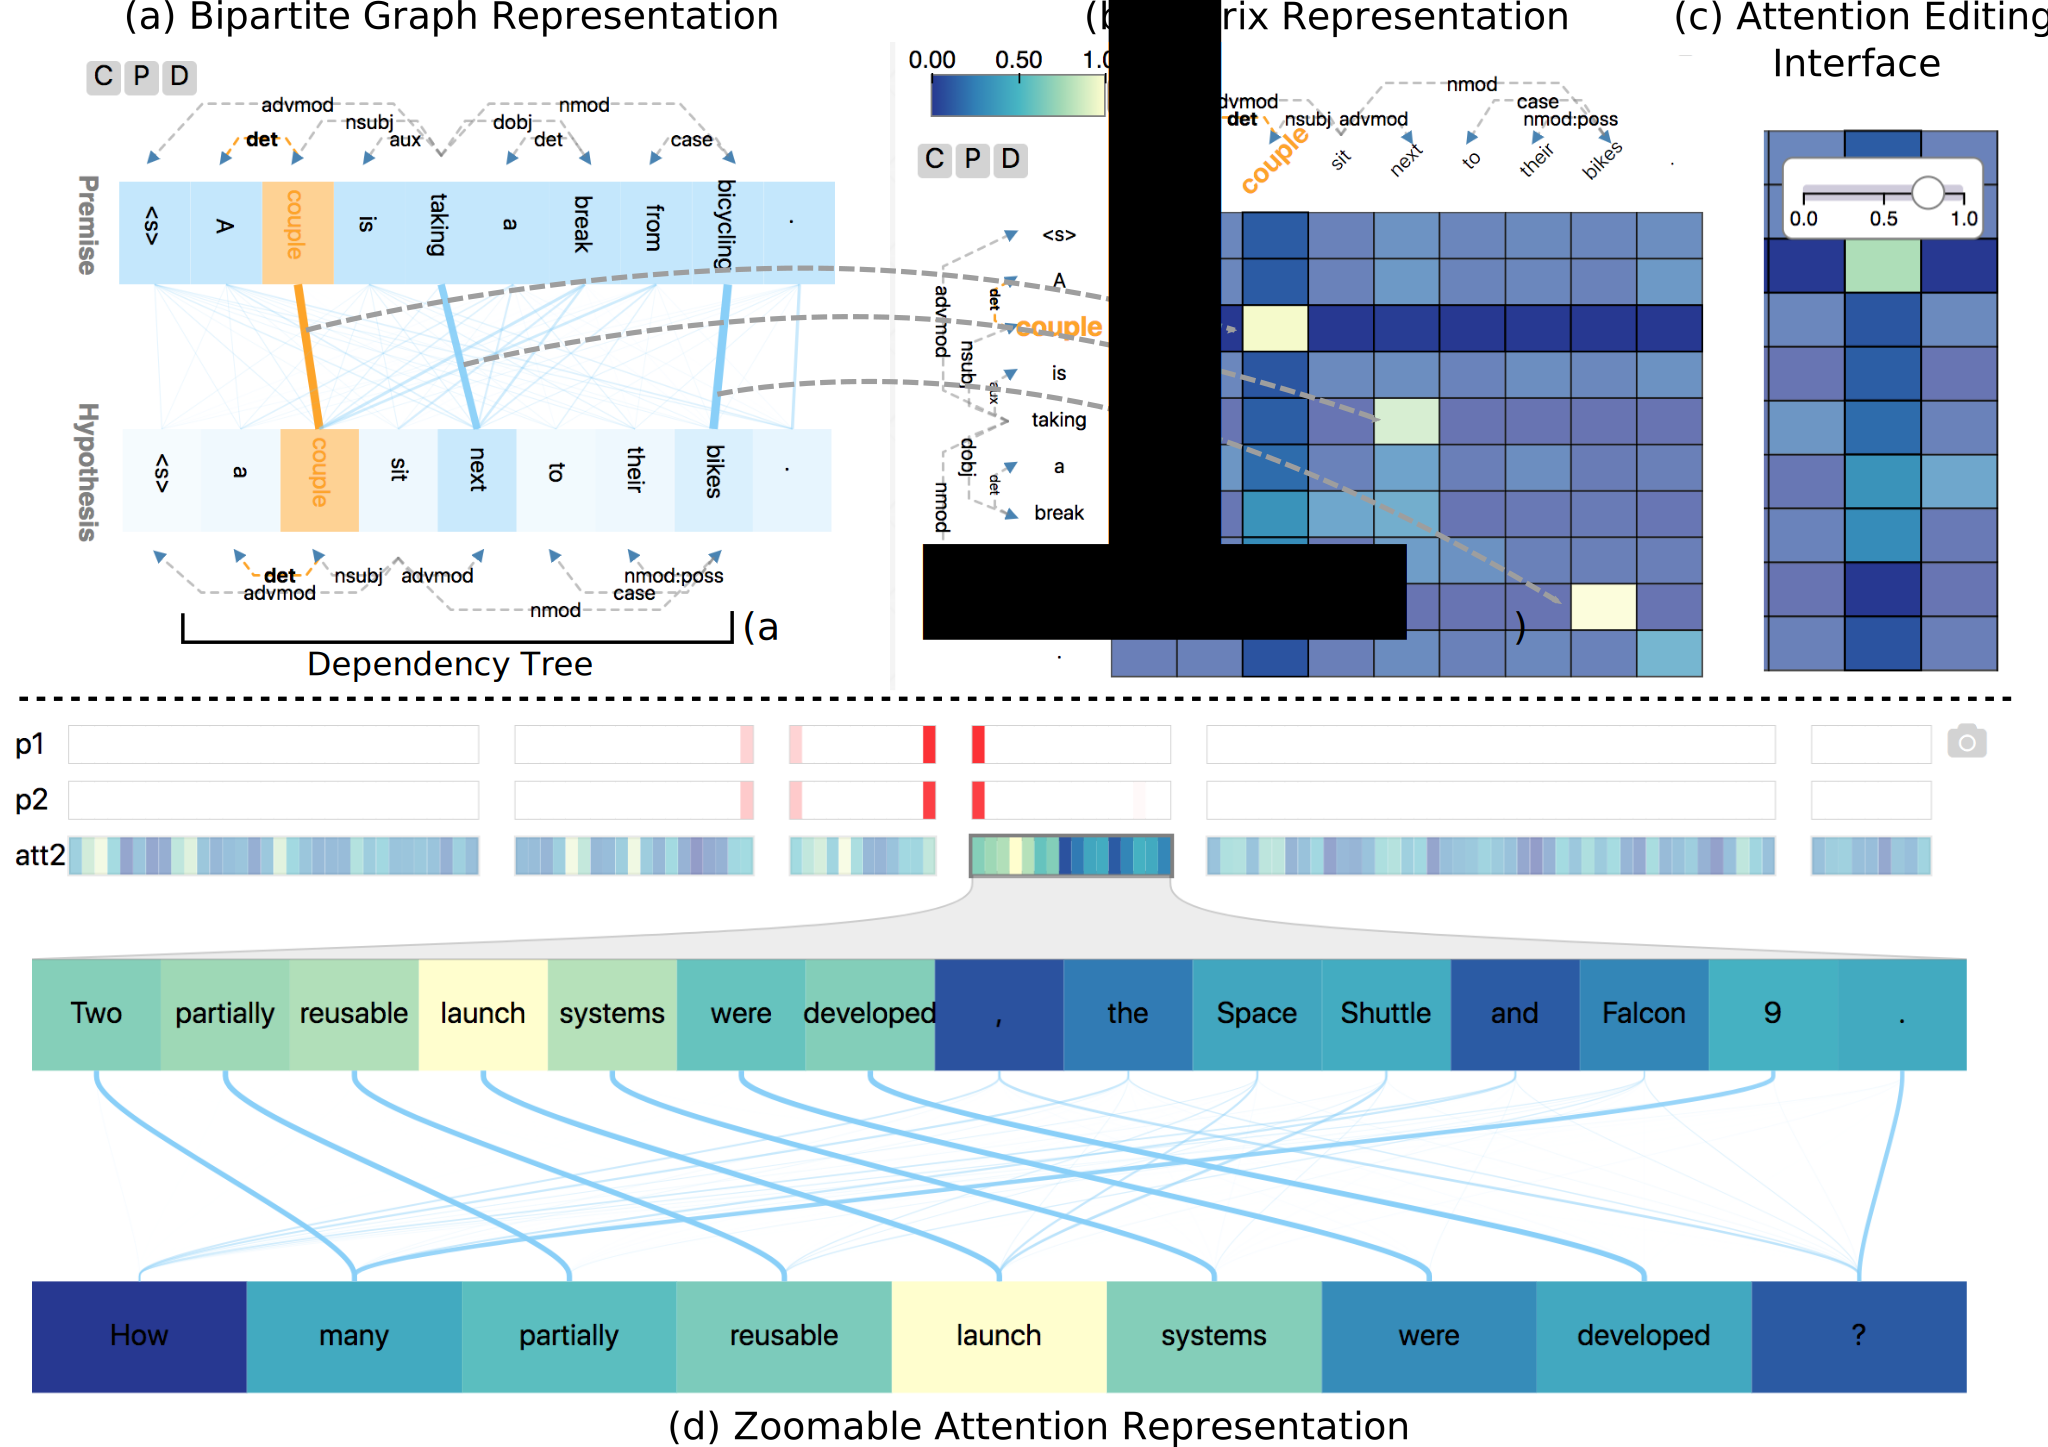
\includegraphics[width=1.0\linewidth]{attentionPanels}
  \vspace{-6mm}
 \caption{
Attention visualization. In the graph attention view (a), a bipartite graph encoding is adopted, in which the edge thickness corresponds to the attention value. In the matrix attention view (b), the entries of $i^{th}$ row represent the probabilities of words in hypotheses align to the $i^{th}$ word in the premise.
The user can alter the attention values via the pop-up interface illustrated in (c).
We overlay the dependency tree ($a_1$) grammar structure to highlight important words and allow simplification of complex sentence based on the dependency tree.
%
For highly asymmetric attention relationship, we utilized a zoomable hierarchical visual representation (d).
}
\label{fig:attention}
\end{figure*}

\subsection{Attention Views}
As illustrated in Figure~\ref{fig:attention}(a)(b), the most widely adopted technique to bipartie graph

Attention matrix


\subsection{Perturbation based exploration}
\label{sec:perturb}

\subsection{Prediction Summarization}



